\documentclass[11pt,a4paper]{article}
\usepackage[margin=2.2cm]{geometry}
\usepackage{graphicx,booktabs,url,amsmath}
\usepackage[hidelinks]{hyperref}
\usepackage{placeins}
\usepackage{float}
\graphicspath{{../../../fullsim_analysis/results/bench/2026-10-27/}}
\newcommand{\results}{../../../fullsim_analysis/results/bench/2026-10-27}
\title{Single-photoelectron calibration of the Citiroc front end:\\ menu 3 of 27 October 2026}
\author{J.\,J.~Gómez-Cadenas}
\date{28 October 2026}
\begin{document}
\maketitle

\begin{center}
\small
\begin{tabular}{lp{0.72\textwidth}}
\toprule
session & 27 October 2026, menu 3 of the Citiroc~1A calibration programme \\
boards & 1, 2 and 4 (A5202, CAEN adapter boards, FPGA firmware 0xa7070800) \\
SiPMs & 43, 42 and 41~V \\
measurements & five runs with the periodic trigger at three biases and three shaping times;
  three staircases of board 1 at 43 and 41~V \\
this report & gain of every channel in ADC counts per photoelectron against bias and
  shaping; breakdown voltage of every channel; pedestal noise of menu~1 in photoelectrons;
  photoelectron spacing of the staircases \\
\bottomrule
\end{tabular}
\end{center}

\section{Goal}

\begin{itemize}
\item The simulation expresses every charge in photoelectrons; the chip stores ADC counts.
  The gain of a channel, in counts per photoelectron, is the unit of the whole chain.
\item With the SiPMs above breakdown and a periodic trigger, the window of the peak detector
  opens at a random time: it holds the pedestal, or the dark pulse of 1, 2, 3~pe that fell
  inside. The spectrum of the channel is a ladder of equally spaced peaks, and the spacing is
  the gain.
\item Menu 3 measures, for every channel of every board:
  \begin{itemize}
  \item the gain at three biases and, at the highest, at three shaping times;
  \item the breakdown voltage, from the gain against the bias;
  \item the pedestal noise of menu~1 in photoelectrons, with the gain just measured.
  \end{itemize}
\item The staircases at two biases give the size of one photoelectron in units of the
  threshold at each.
\end{itemize}

\section{Data}

\begin{itemize}
\item Runs: five (Table~\ref{tab:runs}), periodic trigger at 1~kHz, HoldDelay 200~ns,
  50\,000 events per board.
\item SiPMs: 43, 42 and 41~V (the output of the HV module minus the 4.2~V of the individual
  adjustment).
\item Citiroc: preamplifier gains 55; peak-stretch mode; high gain at 25, 50 or 87.5~ns.
\item Staircases (scans 113 to 115): board 1, trigger rate of each channel against the
  threshold of its discriminator, 25~ns, 0.5~s per point.
\end{itemize}

\begin{table}[H]
\centering
\small
\begin{tabular}{llll}
\toprule
Run & Bias at the SiPM & HG shaping & Boards \\
\midrule
108, 109, 110 & 43 V & 25, 50, 87.5 ns & 1, 2, 4 \\
111 & 42 V & 25 ns & 1, 2, 4 \\
112 & 41 V & 25 ns & 1, 2, 4 \\
\midrule
Scan & Bias at the SiPM & Thresholds & Board \\
\midrule
113 & 43 V & 184--385 & 1 \\
114, 115 & 41 V & 150--300, 190--275 & 1 \\
\bottomrule
\end{tabular}
\caption{Runs and staircases of menu 3, 27 October.}
\label{tab:runs}
\end{table}

\section{Method}

\begin{itemize}
\item With the periodic trigger the window of 200~ns opens at a random time with respect to the
  dark pulses of the channel: the spectrum of a channel is a ladder of peaks at 0, 1, 2, \ldots
  photoelectrons.
\item The spectrum of each channel is fitted with a comb of six Gaussians,
  \begin{equation*}
  f(x) = \sum_{n=0}^{5} A_n \exp\left[-\frac{(x - p - n g)^2}{2(\sigma_0^2 + n\sigma_1^2)}\right],
  \end{equation*}
  with $p$ the 0-pe peak, $g$ the gain in ADC counts per photoelectron, $\sigma_0$ the width of
  the 0-pe peak and $\sigma_1$ the extra width per photoelectron.
\item Seed of $g$: the peaks of the spectrum at 41~V, then the gain at the previous bias scaled
  by the overvoltage.
\item The ladder is resolved when $\sqrt{\sigma_0^2 + \sigma_1^2} < g / 2$.
\item Breakdown voltage of a channel: intercept of the line through its gain at 41, 42 and 43~V.
\item Left out: the six channels without signal from their SiPM (61 and 63 of board~1; 3, 59,
  61 and 63 of board~4).
\end{itemize}

\section{Results}

\subsection{Ladders and gains}

\begin{figure}[H]
\centering
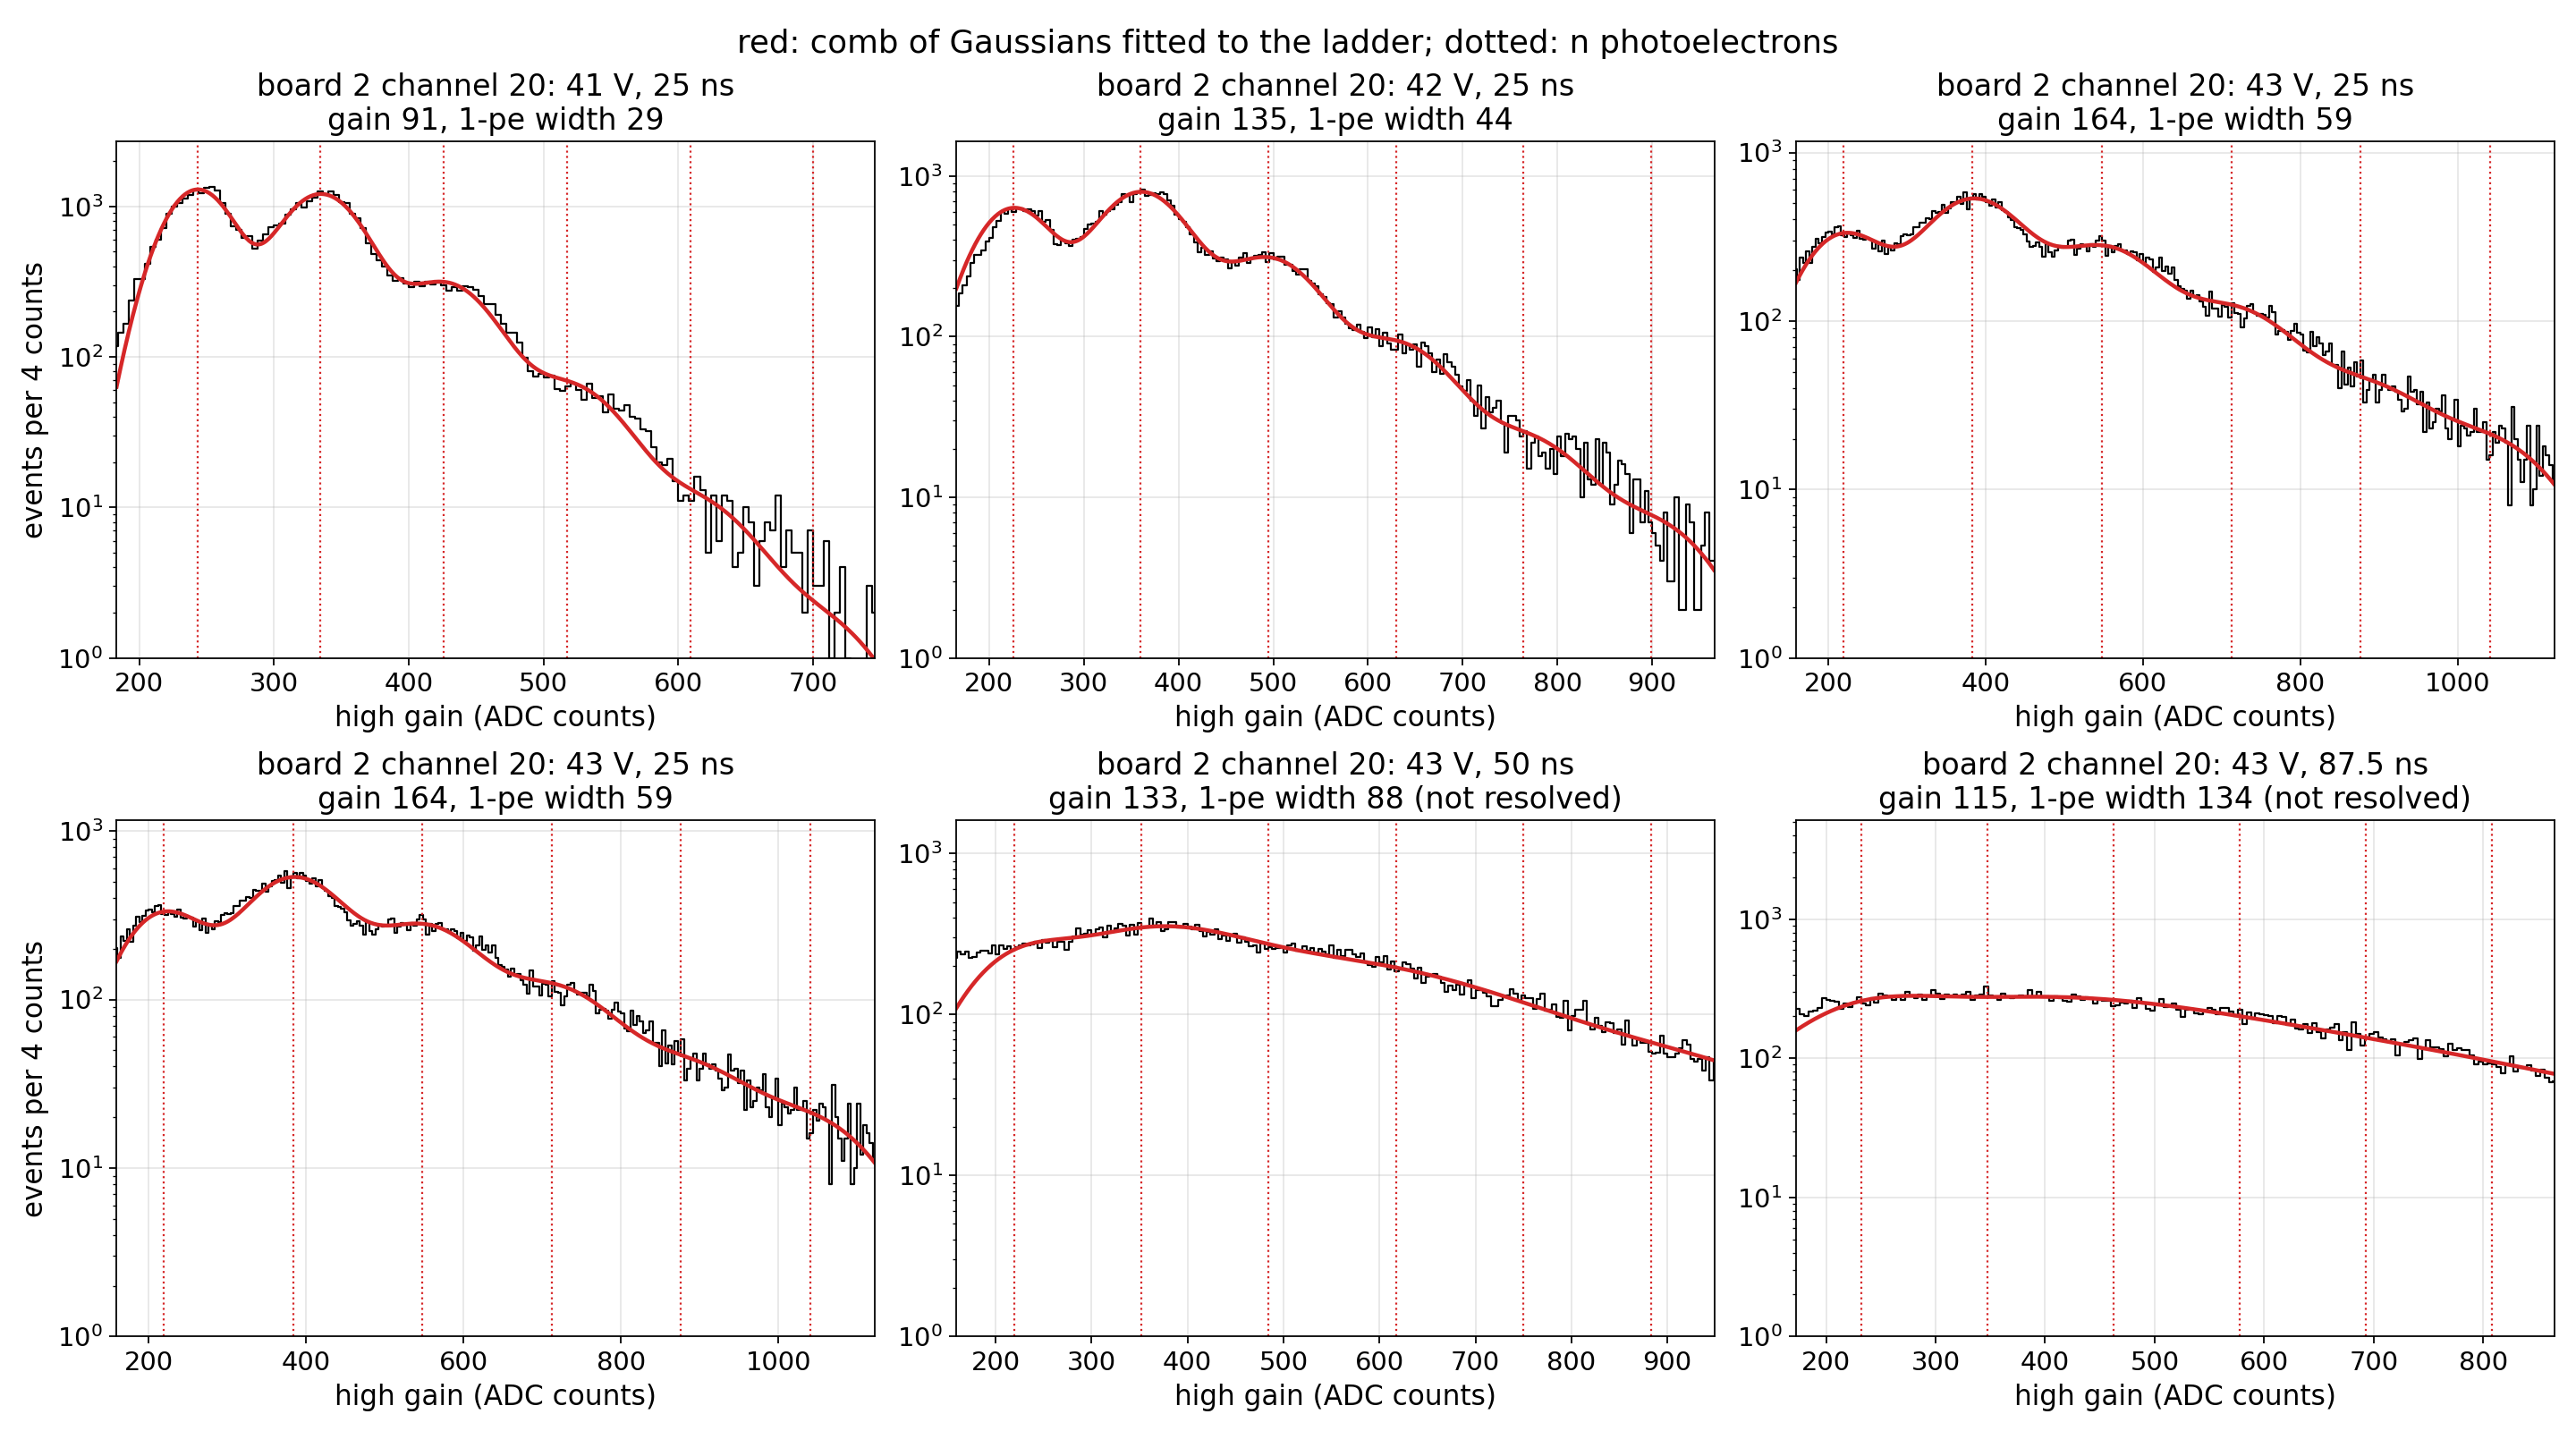
\includegraphics[width=\textwidth]{spe_spectra.png}
\caption{Channel 20 of board 2: the spectrum of the high gain at 41, 42 and 43~V with 25~ns of
shaping (top) and at 43~V with 25, 50 and 87.5~ns (bottom), with the comb of Gaussians fitted
to the ladder.}
\label{fig:spectra}
\end{figure}

\begin{figure}[H]
\centering
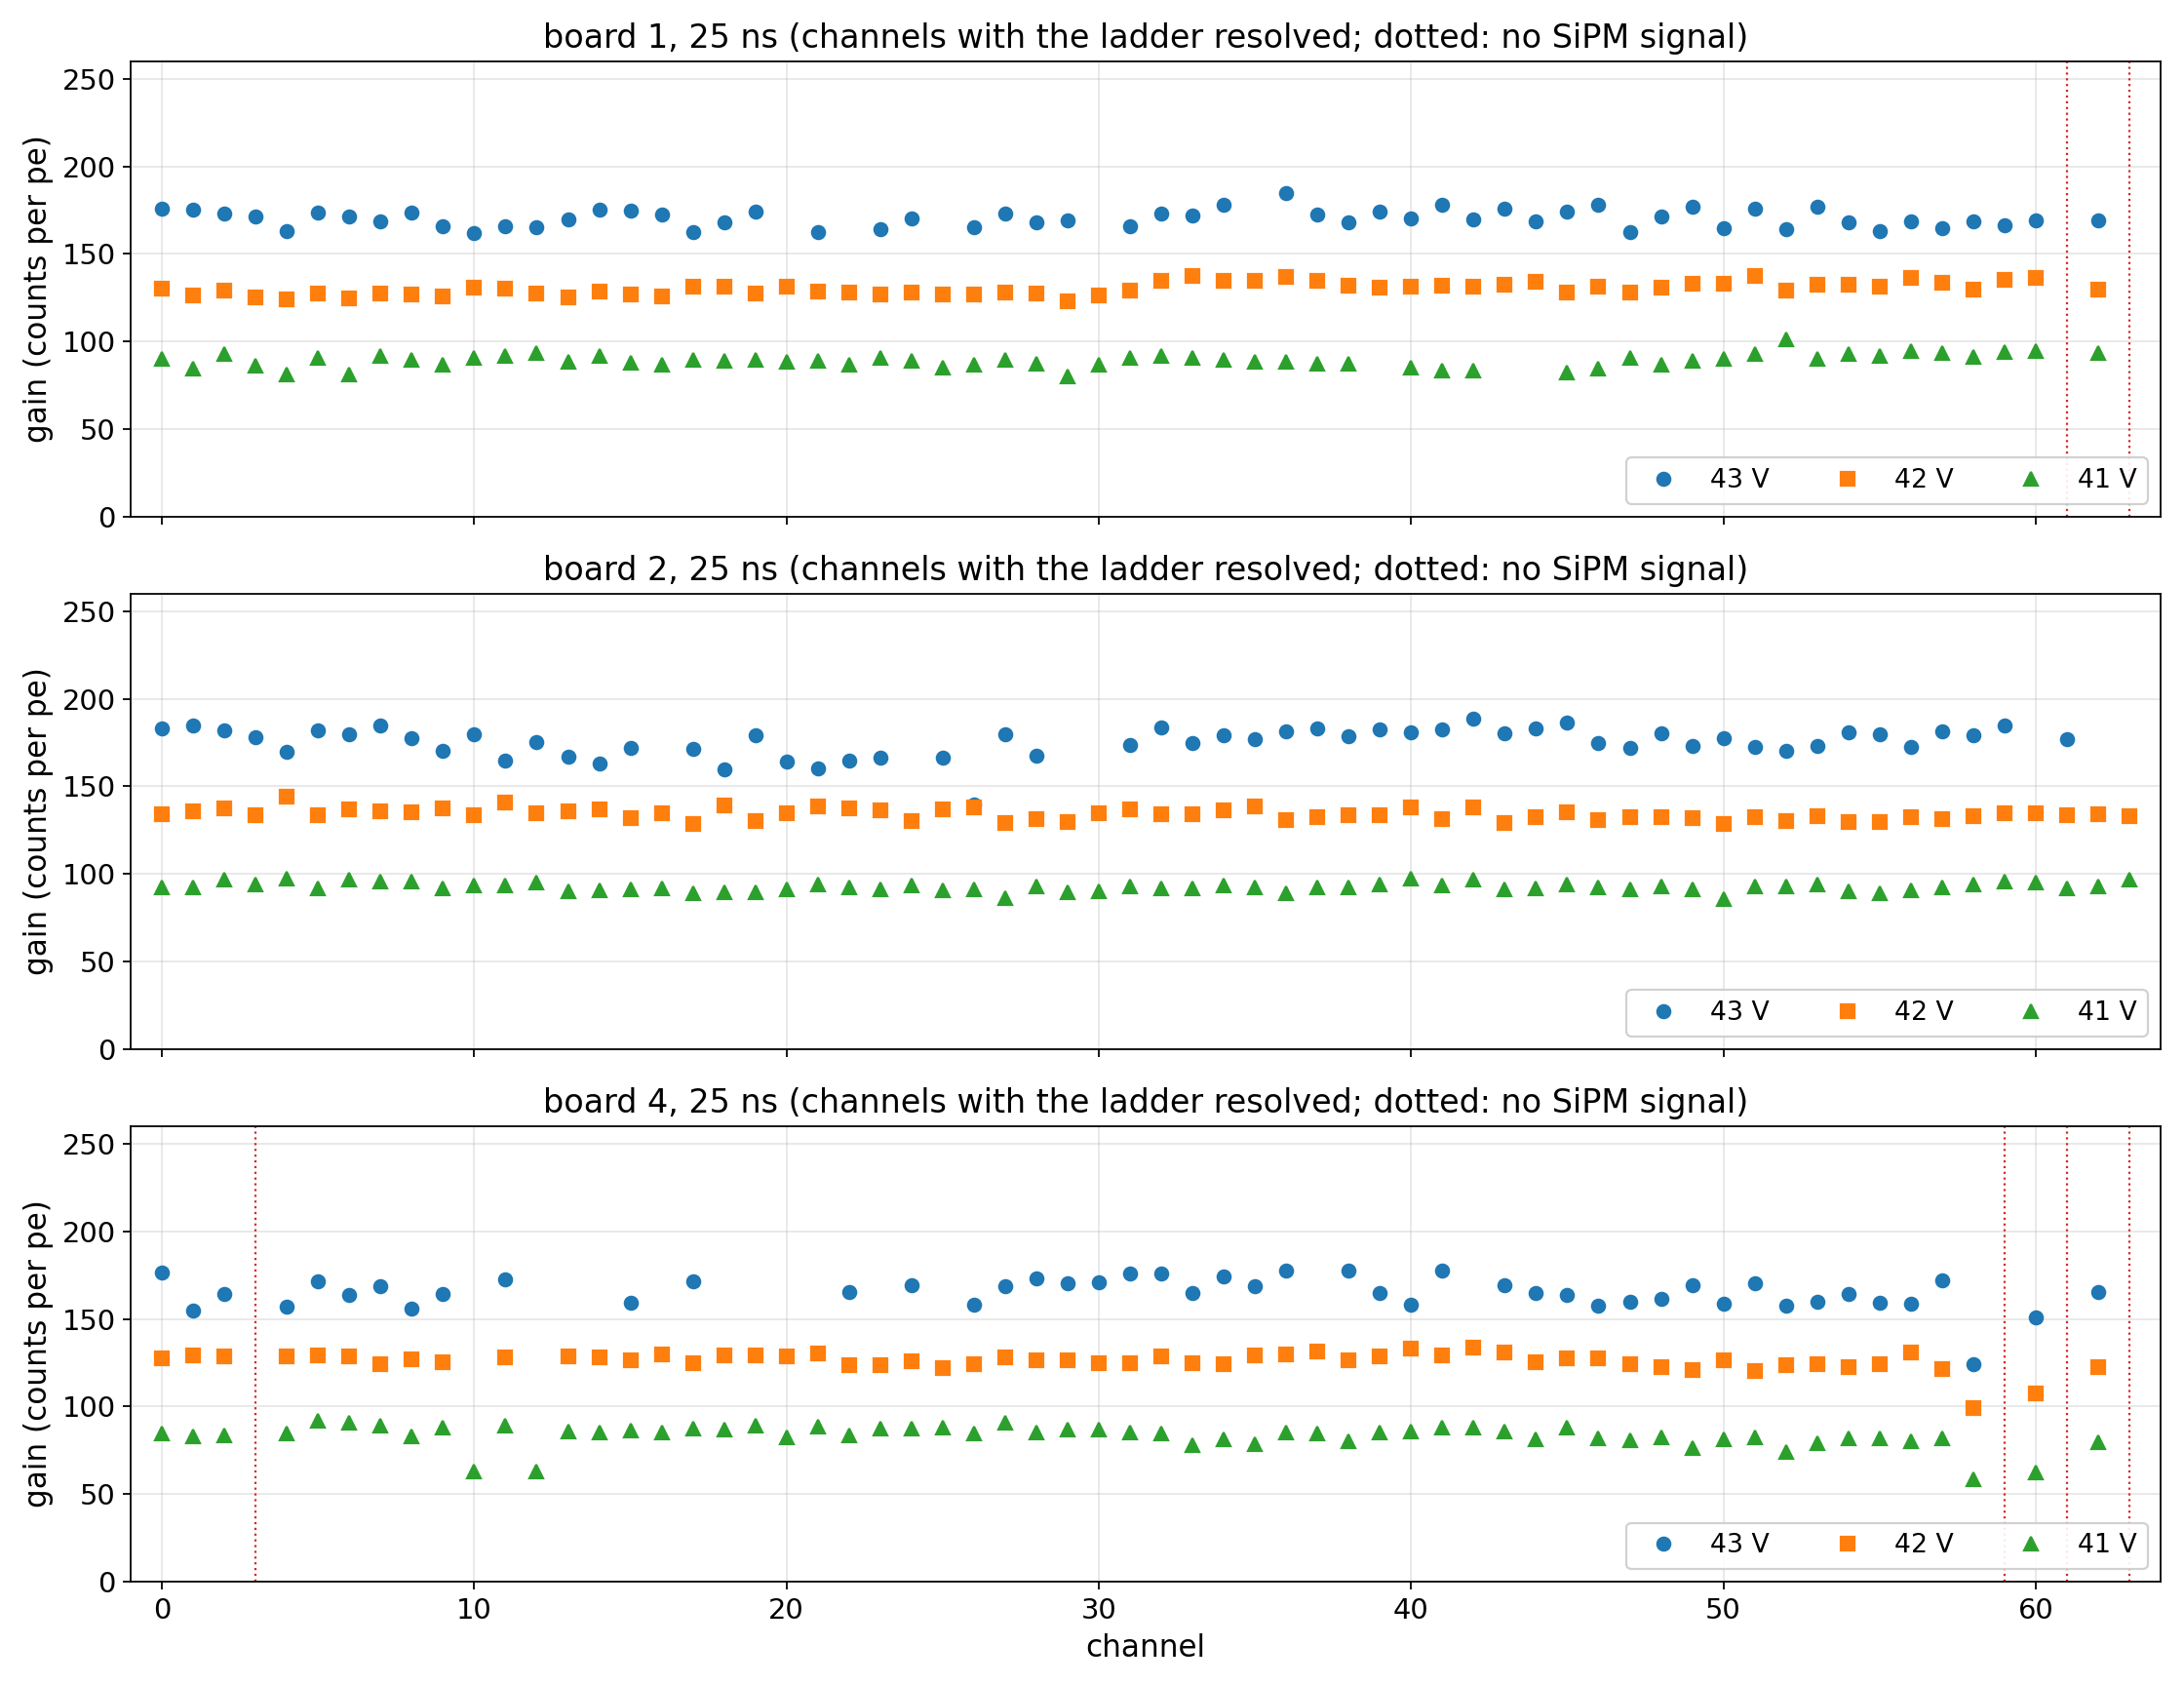
\includegraphics[width=0.95\textwidth]{spe_gains.png}
\caption{Gain of every channel of the three boards at 41, 42 and 43~V, 25~ns of shaping;
channels with the ladder resolved.}
\label{fig:gains}
\end{figure}

\begin{table}[H]
\centering
\small
\input{\results/spe_gains_table.tex}
\caption{Per board, bias and shaping: channels with the ladder resolved, median and range of
the gain, and median width of the 1-pe peak, in ADC counts of the high gain.}
\label{tab:gains}
\end{table}

\begin{itemize}
\item Ladder resolved at 25~ns in 183, 184 and 161 of the 186 channels at 41, 42 and 43~V
  (Figure~\ref{fig:spectra}, Table~\ref{tab:gains}).
\item Gain, medians of the three boards: 85--92 counts per photoelectron at 41~V, 127--134 at
  42~V, 165--178 at 43~V (Figure~\ref{fig:gains}).
\item Spread across the channels of a board (rms over median): 2.4--5.6\%.
\item Width of the 1-pe peak: 25--30 counts at 41~V, 49--52 at 43~V.
\end{itemize}

\subsection{Gain against bias and breakdown voltage}

\begin{figure}[H]
\centering
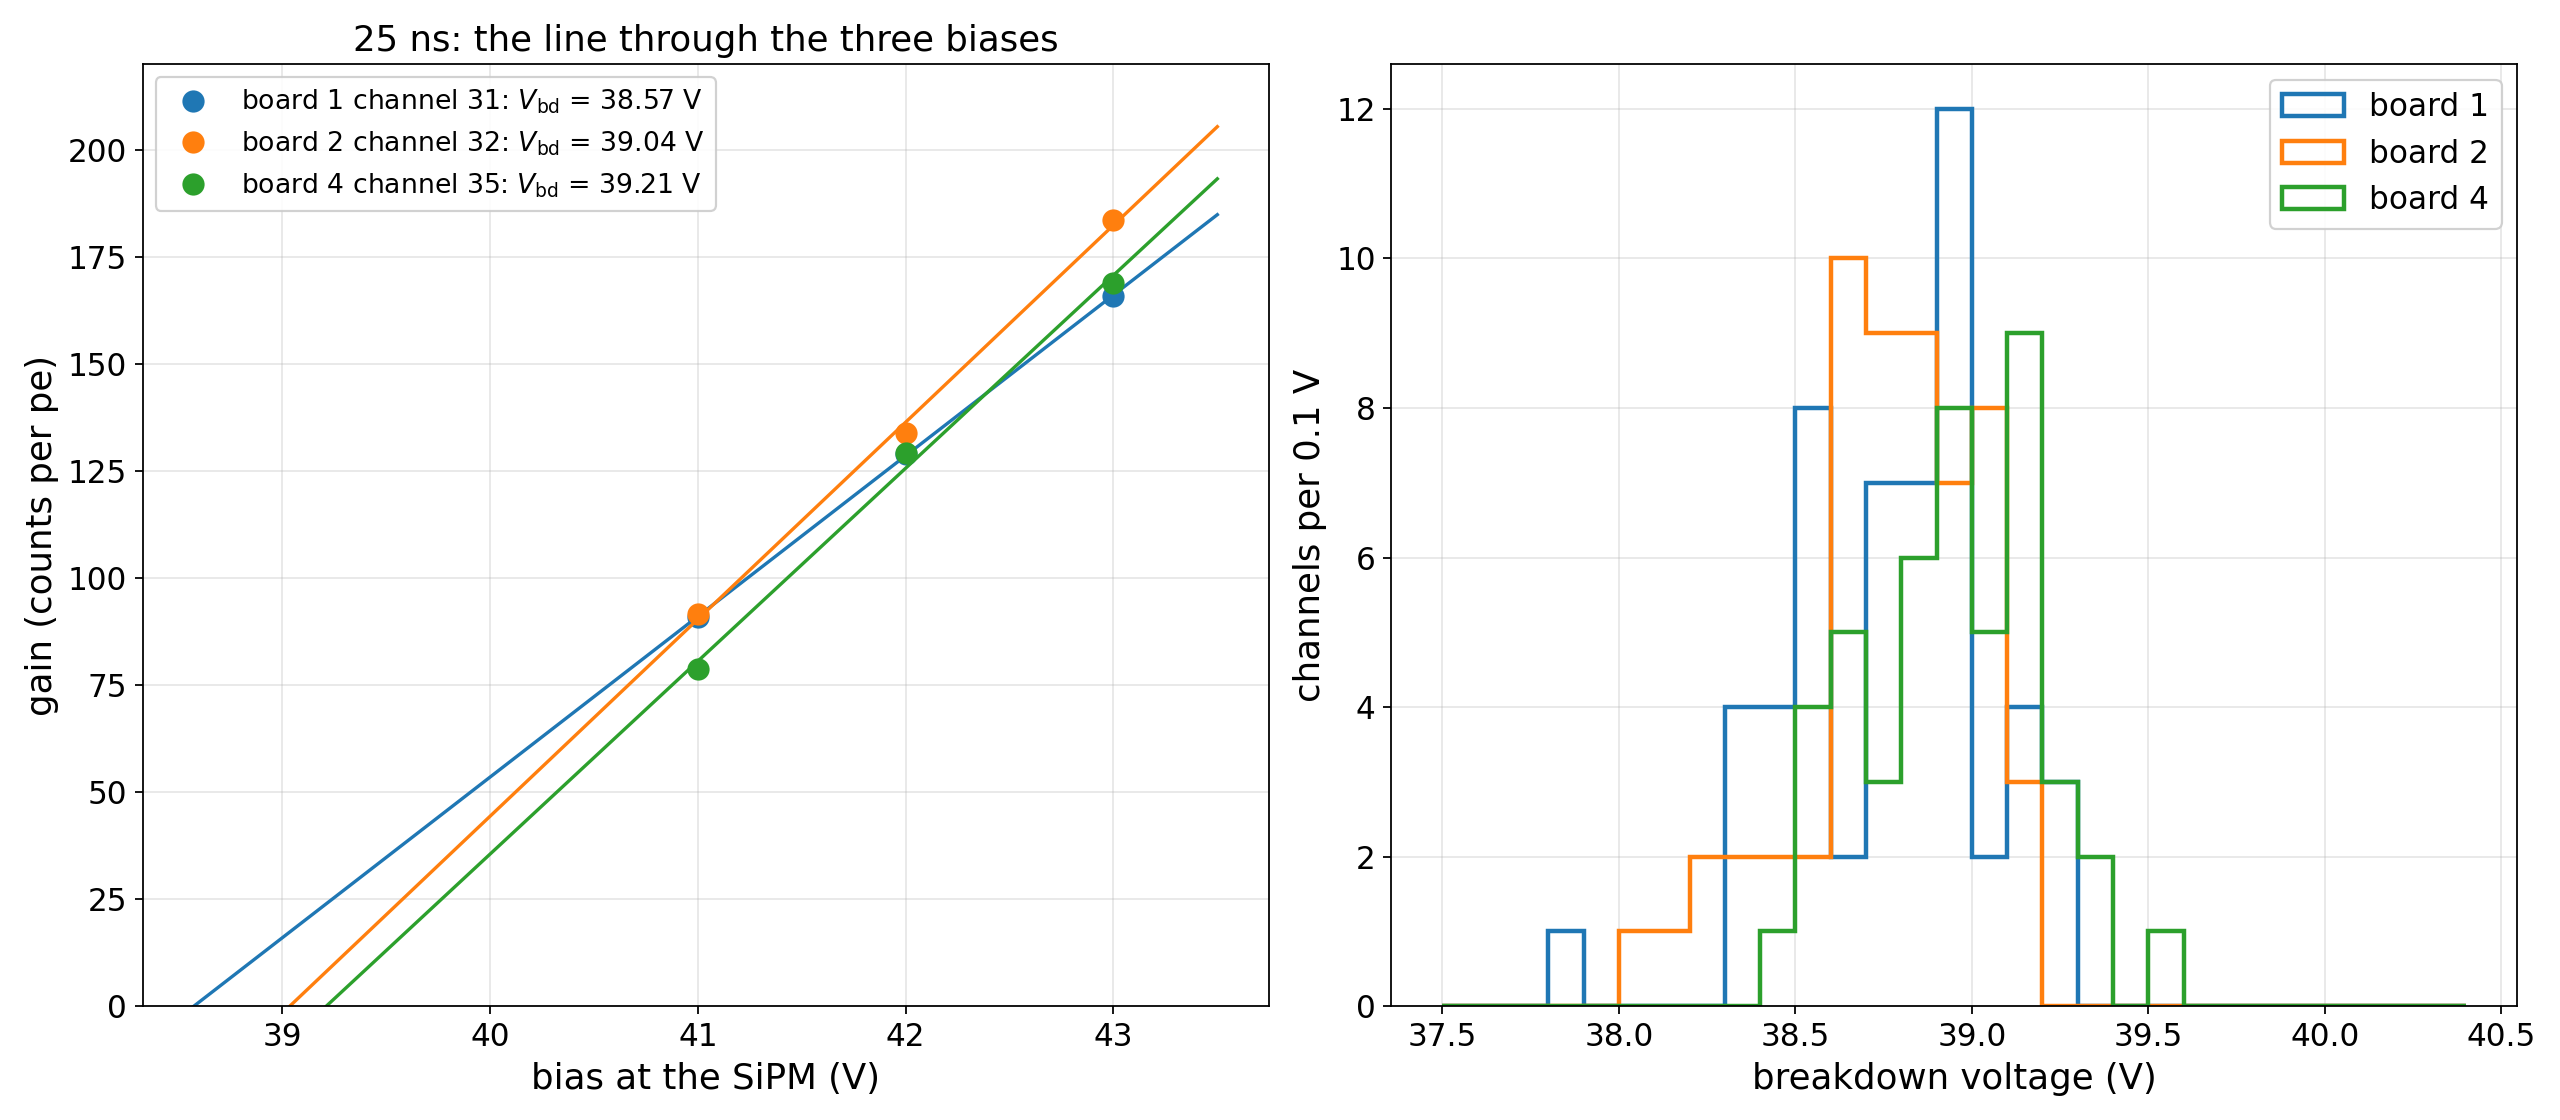
\includegraphics[width=\textwidth]{spe_breakdown.png}
\caption{Left: gain against bias for one channel of each board, with the fitted line. Right:
distribution of the breakdown voltage of the channels of each board.}
\label{fig:breakdown}
\end{figure}

\begin{table}[H]
\centering
\small
\input{\results/spe_breakdown_table.tex}
\caption{Per board: channels with the three biases resolved, median and range of the breakdown
voltage and of the slope of the gain, and the detector temperature recorded by the board.}
\label{tab:breakdown}
\end{table}

\begin{itemize}
\item $g = a\,(V - V_\mathrm{bd})$ (Figure~\ref{fig:breakdown}, left): $a$ = 41--42 counts per
  photoelectron per volt.
\item $V_\mathrm{bd}$ = 38.8, 38.8, 39.0~V (medians of boards 1, 2, 4), rms 0.25--0.35~V across
  the channels of a board (Table~\ref{tab:breakdown}).
\item Overvoltage at 43, 42 and 41~V: 4.1, 3.1 and 2.1~V (4.0--4.2~V at 43~V).
\end{itemize}

\subsection{Gain against shaping}

\begin{figure}[H]
\centering
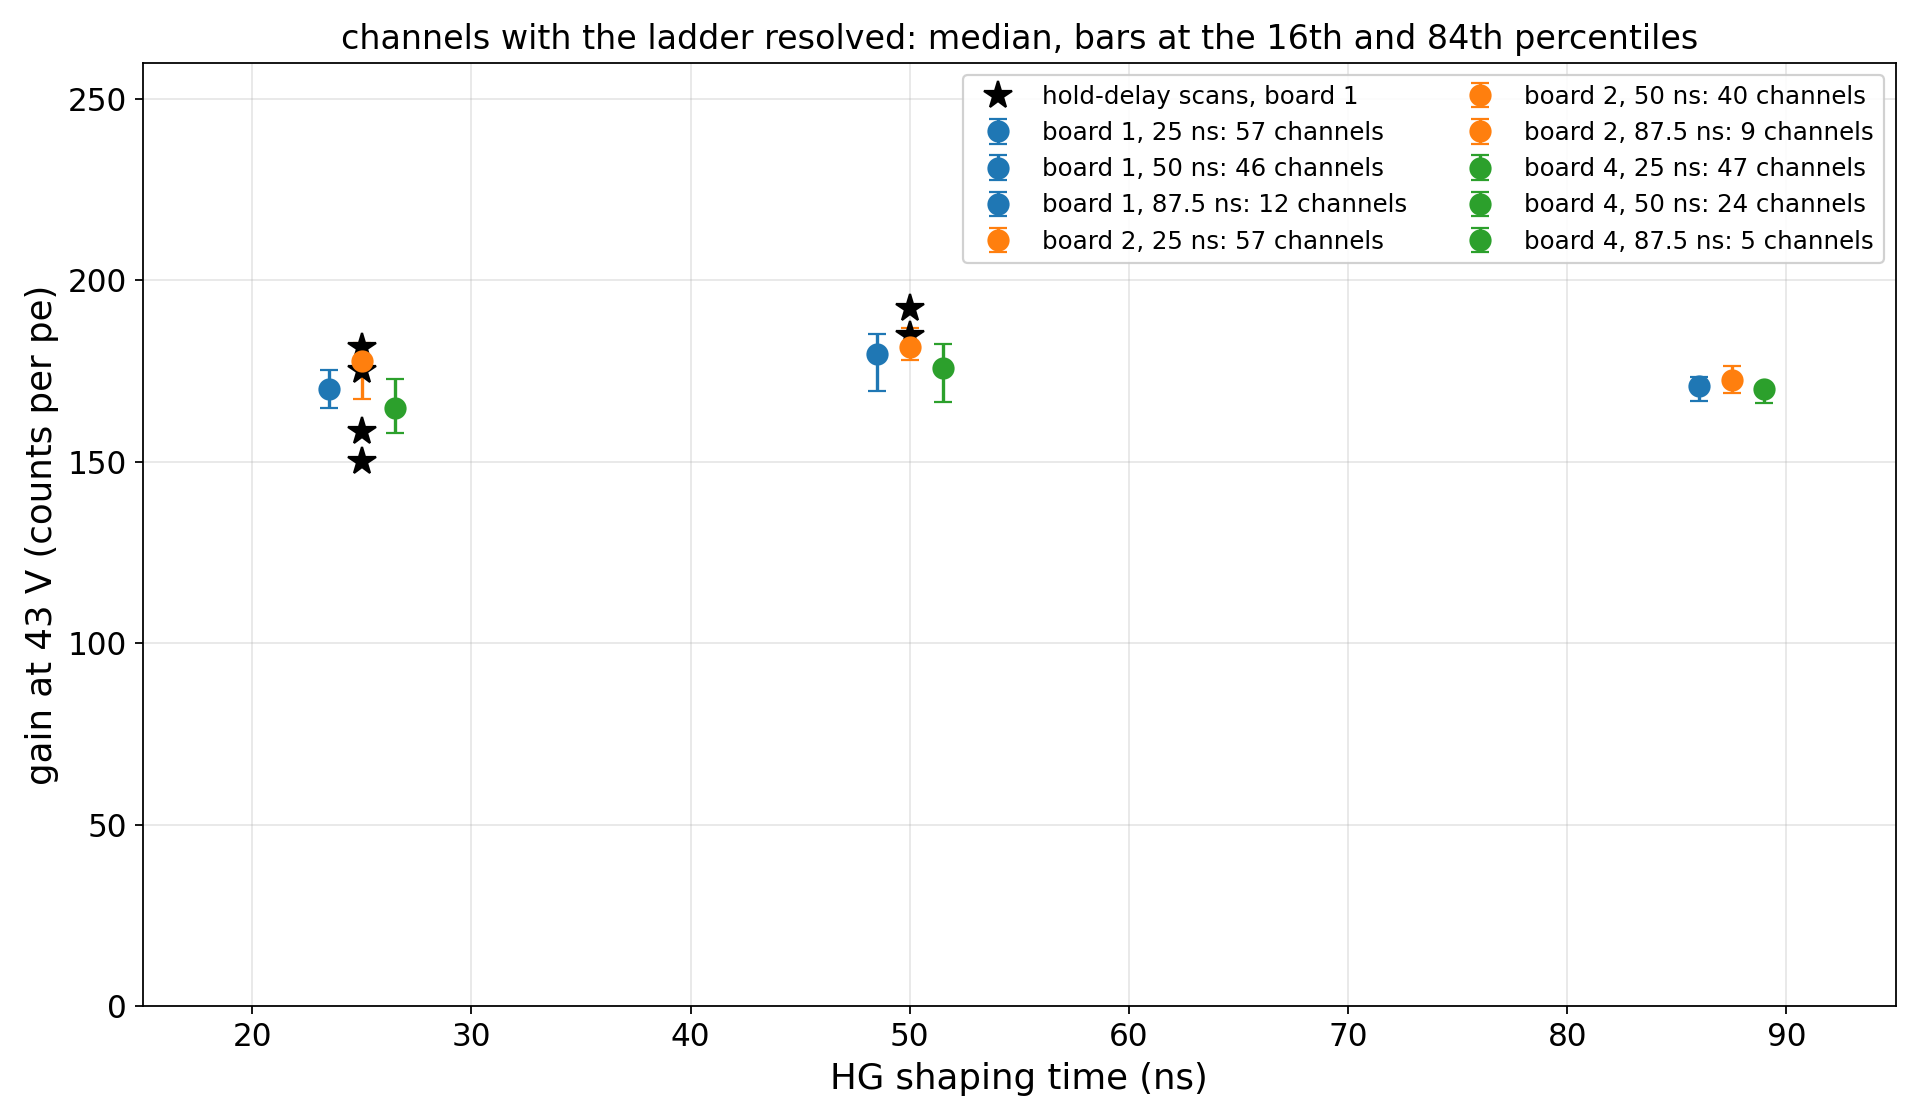
\includegraphics[width=0.8\textwidth]{spe_shaping.png}
\caption{Gain at 43~V against the shaping time: median over the channels with the ladder
resolved, bars at the 16th and 84th percentiles; stars, the plateau of the 1-pe peak in the
hold-delay scans of board 1 (menu 2).}
\label{fig:shaping}
\end{figure}

\begin{itemize}
\item Ladder resolved at 43~V in 110 channels at 50~ns and 26 at 87.5~ns (1-pe width
  61--67 counts).
\item Gain at 43~V: 165--178 at 25~ns, 176--182 at 50~ns, 170--173 at 87.5~ns
  (Figure~\ref{fig:shaping}).
\item Menu 2 against menu 3, board 1, 43~V: channels 0, 40, 60 at 25~ns, 175, 159, 182 against
  176, 170, 169; channel 0 at 50~ns, 185 and 192 against 187. Channel 20: ladder not resolved.
\end{itemize}

\subsection{Noise in photoelectrons}

\begin{figure}[H]
\centering
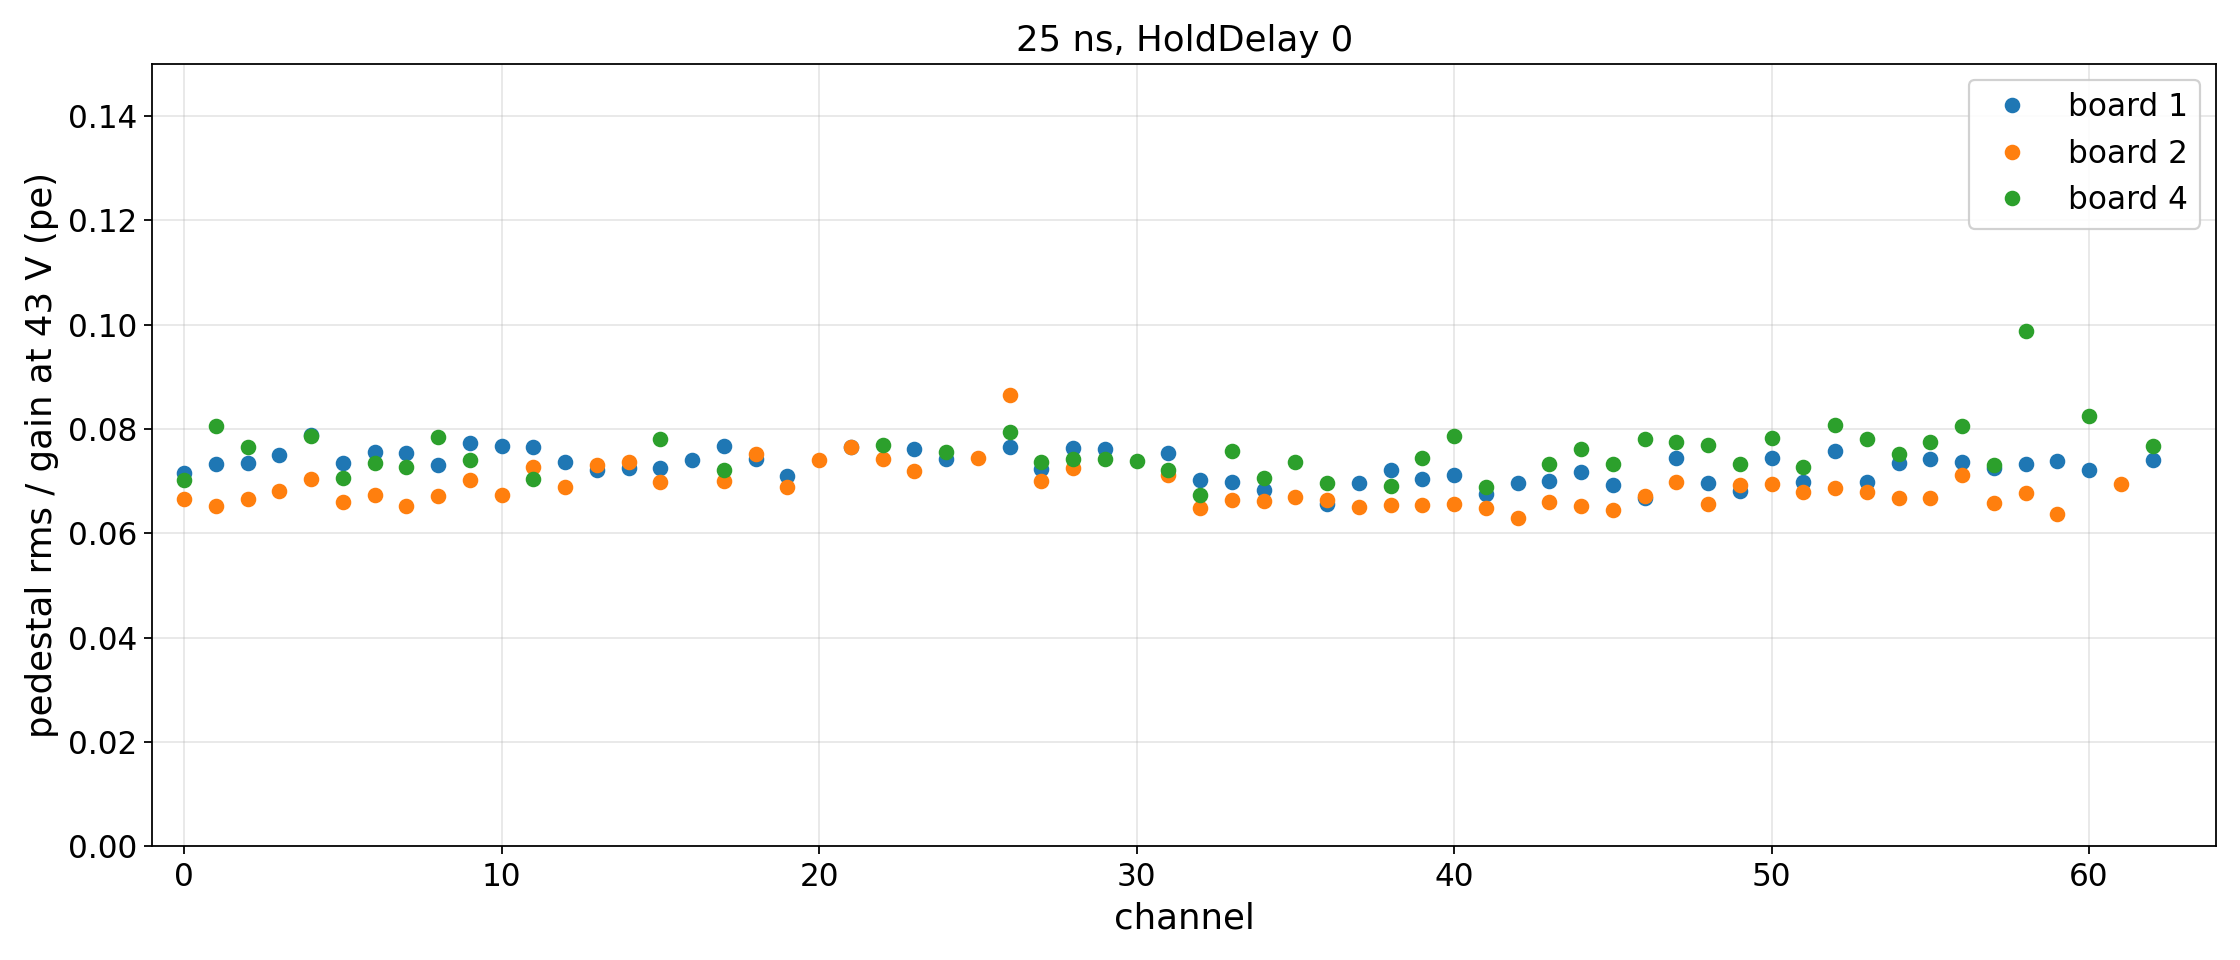
\includegraphics[width=0.9\textwidth]{spe_noise_pe.png}
\caption{Pedestal noise of every channel (menu 1, 25~ns, HoldDelay 0) divided by its gain at
43~V.}
\label{fig:noisepe}
\end{figure}

\begin{table}[H]
\centering
\small
\input{\results/spe_noise_pe.tex}
\caption{Per board and shaping: median gain at 43~V, total, coherent and incoherent pedestal
noise of menu 1 (HoldDelay 0) in ADC counts and in photoelectrons.}
\label{tab:noisepe}
\end{table}

\begin{itemize}
\item Noise in photoelectrons: $\sigma / g$, with $\sigma$ the pedestal noise of menu~1 at
  HoldDelay 0 and $g$ the median gain of the board at 43~V and the same shaping.
\item 25~ns: 0.068--0.075 photoelectrons per channel, 0.033--0.038 coherent, 0.059--0.065
  incoherent (Table~\ref{tab:noisepe}, Figure~\ref{fig:noisepe}).
\item 50~ns: 0.067--0.074, coherent 0.041--0.046.
\end{itemize}

\subsection{Staircases at 5 and 3 V}

\begin{table}[H]
\centering
\small
\input{\results/spe_staircases.tex}
\caption{Staircases of board 1: bias, edge of the noise of the fast shaper, spacing of the
photoelectron steps and dark rate 30 DAC units above the edge, medians over the channels with
their ranges.}
\label{tab:staircases}
\end{table}

\begin{itemize}
\item Edge of the noise: 190 DAC units at 43~V, 182 at 41~V (Table~\ref{tab:staircases}; scan
  115 starts above the edge).
\item Photoelectron steps: 22 units at 43~V, 12.5 at 41~V; ratio 1.8, as the gains.
\item One DAC unit of the threshold: 7.8 counts of the high gain at 43~V, 7.1 at 41~V.
\item Dark rate 30 units above the edge: $1.4\times 10^{5}$~Hz at 43~V, $2.8\times 10^{3}$~Hz at
  41~V.
\end{itemize}

\subsection{Entries at zero}

\begin{table}[H]
\centering
\small
\input{\results/spe_zeros.tex}
\caption{Fraction of the high-gain entries at 0, in percent, median over the channels of each
board.}
\label{tab:zeros}
\end{table}

\begin{itemize}
\item High-gain entries at 0 (Table~\ref{tab:zeros}): 0.5--1.1\% at 43~V and 25~ns, 3.8--6.1\%
  at 50~ns, 8.9--12.0\% at 87.5~ns; 0.1\% or less at 42~V; none at 41~V.
\item The pedestal runs of menu~1 have no entry at 0.
\item The fits leave these entries out; their origin is open (finding F12).
\end{itemize}

\section{Summary of results}

Main findings:
\begin{itemize}
\item At 25~ns the ladder of dark pulses is resolved in nearly every channel (183, 184 and
  161 of 186 at 41, 42 and 43~V); at 50~ns in 110 channels; at 87.5~ns in 26, because the
  dark pulses pile up in the longer shaping.
\item The gain is linear in the bias, 41--42 counts per photoelectron per volt, and the
  breakdown voltage is 38.8--39.0~V on the three boards, uniform within 0.3~V across the
  channels. The bias of 43~V is 4.1~V above breakdown, not 5.
\item The gain varies by 2.4--5.6\% across the channels of a board and little with the
  shaping (165--182 counts per photoelectron at 43~V).
\item The pedestal noise of the chain at 43~V and 25~ns is 0.07 photoelectrons per channel,
  half of it coherent.
\item One DAC unit of the threshold is 7.8 counts of the high gain at 43~V; one photoelectron
  is 22 units at 43~V and 12.5 at 41~V.
\item Open: at 43~V a fraction of the entries, growing with the shaping from 0.5 to 12\%,
  reads 0 (finding F12).
\end{itemize}

\begin{table}[H]
\centering
\small
\begin{tabular}{p{0.3\textwidth}p{0.55\textwidth}}
\toprule
gain, 25 ns, high gain, preamplifier gain 55 & 85--92 counts per photoelectron at 41~V,
  127--134 at 42~V, 165--178 at 43~V (medians of the three boards); spread across the channels
  of a board 2.4--5.6\% \\
gain at 43 V against shaping & 165--178 at 25~ns, 176--182 at 50~ns, 170--173 at 87.5~ns \\
breakdown voltage & 38.8, 38.8, 39.0~V (boards 1, 2, 4), rms 0.25--0.35~V across the
  channels; 41--42 counts per photoelectron per volt; 43~V is 4.0--4.2~V above breakdown \\
pedestal noise at 43 V, 25 ns, HoldDelay 0 & 0.068--0.075 photoelectrons per channel,
  0.033--0.038 coherent, 0.059--0.065 incoherent \\
threshold & one photoelectron = 22 DAC units at 43~V, 12.5 at 41~V; edge of the noise at
  190 and 182 \\
entries at 0, 43 V & 0.5--1.1\% at 25~ns, 3.8--6.1\% at 50~ns, 8.9--12\% at 87.5~ns \\
\bottomrule
\end{tabular}
\caption{Values: gains, breakdown voltages, noise in photoelectrons, threshold units.}
\label{tab:values}
\end{table}

\end{document}
